\section*{Aufgabe 4}
\subsection*{a)}
\begin{multicols}{2}
	\raggedright
	Algorithmus X:\\
	\begin{center}
		\begin{tabular}{|c|c|c|}\hline
			& Pos. Pred. &Neg. Pred.\\\hline
			True Failure &2& 3\\\hline
			No Failure&3&95\\\hline
		\end{tabular}\\
	\end{center}
\columnbreak
	Algroithmus Y:\\
	\begin{center}\begin{tabular}{|c|c|c|}\hline
			& Pos. Pred. &Neg. Pred.\\\hline
			True Failure &2& 4\\\hline
			No Failure&4&93\\\hline
		\end{tabular}
	\end{center}
\end{multicols}
\subsection*{b)}
\begin{center}
	\begin{figure}[h]
		\centering
		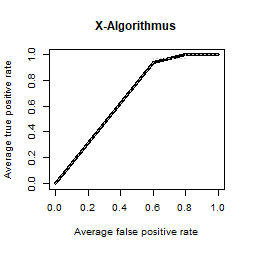
\includegraphics[width=0.45\textwidth]{../4/Screenshots/X.png}
		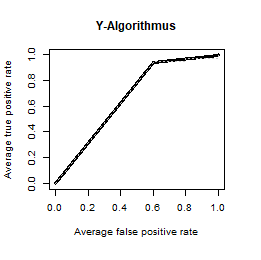
\includegraphics[width=0.45\textwidth]{../4/Screenshots/Y.png}
	\end{figure}
 	Algorithmus X hat eine leicht bessere TPR.
\end{center}

\subsection*{c)}
Höherer Schwellwert $\rightarrow $ Tatsächliche Fehler werden nicht erkannt.
Niedriger Schwellwert $\rightarrow$ Sehr hohes Rauschen, System wird empfindlich
\subsection*{d)}
\centering
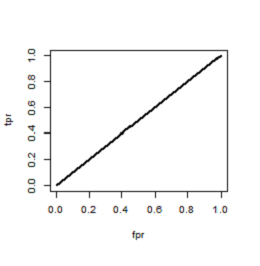
\includegraphics{../4/Screenshots/random.png}